\documentclass[12pt]{article}
% Full article preamble (duplicated, no common file)
\usepackage{fontspec}
\usepackage[a4paper,margin=2.5cm,includefoot]{geometry}
\usepackage{polyglossia}
\usepackage{amsmath}
\usepackage{amssymb}
\usepackage{xcolor}
\usepackage{fancyhdr}
\usepackage{graphicx}
\usepackage{listings}
\usepackage[most]{tcolorbox}
\usepackage{pifont}
\usepackage{enumitem}
\usepackage{titlesec}
\usepackage[bottom]{footmisc}
\usepackage{titling}
\usepackage{minted}
\usepackage{etoolbox}
\usepackage{array}
\usepackage{extsizes}

\newfontfamily\emoji{Segoe UI Emoji}

\pagestyle{fancy}

\setmainlanguage[numerals=western]{arabic}
\setotherlanguage{english}
\newfontfamily\arabicfont[Script=Arabic]{Amiri}
\newfontfamily\arabicfonttt[Script=Arabic]{Courier New}

\lstset{
  language=[Sharp]C,
  numbers=left,
  stepnumber=1,
  numbersep=8pt,
  frame=single,
  basicstyle=\ttfamily\small,
  keywordstyle=\color{blue},
  stringstyle=\color{red},
  commentstyle=\color{green!50!black}
}

\newif\ifdetailed
\ifdefined\setdetailed
  \setdetailed
\fi

\newif\ifwithsols
\ifdefined\setwithsols
  \setwithsols
\fi

% unified tcolorboxes for articles
\tcbset{colback=white, colframe=black, fonttitle=\bfseries, boxrule=0.8pt}
\newtcolorbox{boxDef}[1][]{colback=blue!5!white,colframe=blue!75!black,
  title={{\emoji📘} تعريف\ifx\\#1\\\else ~#1\fi :}}
\newtcolorbox{boxExercise}[1][]{colback=cyan!5!white,colframe=cyan!70!black,
  title={{\emoji🧩} تمرين\ifx\\#1\\\else ~#1\fi :}}
\newtcolorbox{boxExample}[1][]{colback=yellow!5!white,colframe=orange!90!black,
  title={{\emoji📝} مثال\ifx\\#1\\\else ~#1\fi :}}
\newtcolorbox{boxNote}[1][]{colback=gray!10!white,colframe=black,
  title={{\emoji✨} ملاحظة\ifx\\#1\\\else ~#1\fi :}}
\newtcolorbox{boxAttention}[1][]{colback=magenta!10!white,colframe=magenta!80!black,
  title={{\emoji🔔} تنبيه\ifx\\#1\\\else ~#1\fi :}}
\newtcolorbox{boxWarning}[1][]{colback=red!5!white,colframe=red!75!black,
  title={{\emoji⚡} ملاحظة هامة\ifx\\#1\\\else ~#1\fi :}}
\newtcolorbox{boxSolution}[1][]{colback=green!5!white,colframe=green!60!black,
  title={{\emoji✅} حل\ifx\\#1\\\else ~#1\fi :}}
\newtcolorbox{boxSymbol}[1][]{colback=purple!5!white,colframe=purple!70!black,
  title={{\emoji🔣} رمز\ifx\\#1\\\else ~#1\fi :}}

\tcbset{simplecode/.style={ colback=gray!5, colframe=black!50, boxrule=0.4pt, arc=2pt, left=4pt,right=4pt,top=4pt,bottom=4pt}}
\newenvironment{boxCode}{\begin{tcolorbox}[simplecode]}{\end{tcolorbox}}

\newcolumntype{C}[1]{>{\centering\arraybackslash}p{#1}}

% redefine spaces after titles
\makeatletter
\renewcommand{\@maketitle}{%
  \begin{center}
    {\huge \bfseries \@title \par}%
    \vskip 0.2em % space between title and author
    {\large \@author \par}%
    % \vskip 0.2em % space between author and date
    % {\normalsize \@date \par}%
  \end{center}
}
\makeatother

\fancyhf{} % clear default
\fancypagestyle{plain}{
  \fancyhf{}
  \fancyhead[L]{مدرسة التسامح الشاملة}
  % \fancyhead[L]{
\includegraphics[height=1cm]{../../../images/logoTasamoh.png}}
  \fancyhead[R]{الأستاذ محمود اغبارية}
  \fancyfoot[C]{\thepage}
}

\fancyhead[L]{مدرسة التسامح الشاملة}
\fancyhead[R]{الأستاذ محمود اغبارية}
\fancyfoot[C]{\thepage}
% \date{\today}

\setcounter{tocdepth}{3} % only section subsection and subsubsection in TOC


% ----------------------


% \begin{document}

% \maketitle

% % \clearpage  % start TOC on a new page
% % \renewcommand{\contentsname}{جدول المحتويات}
% % \tableofcontents
% % \clearpage

% \part*{part 1} % the * prevents numbering
% \section*{مقدمة}
% \subsection*{مثال رياضي}
% \subsubsection*{مثال فرعي}
% \paragraph*{ paragraph 1}
% \subparagraph*{sub paragraph 1}

% \ifdetailed
% \begin{english}
% \begin{minted}{csharp}
% // C# Example
% \end{minted}
% \end{english}
% \fi

% OLD WAY
% \ifdetailed
% \begin{english}
% \begin{lstlisting}
% // C# Example
% \end{lstlisting}
% \end{english}
% \fi

% % 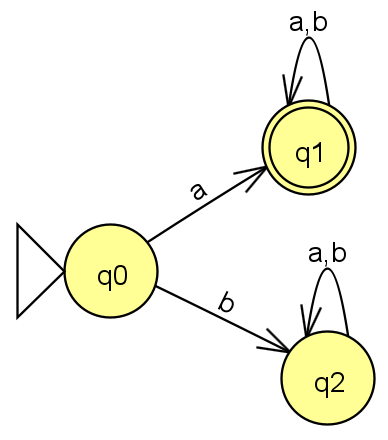
\includegraphics[width=0.2\textwidth]{../../../images/DFAs/ex1_q1.png}



% \vspace{3cm}
% \begin{flushleft}
% أرجو لكم وقتًا ممتعًا.

% الأستاذ محمود اغبارية.
% \end{flushleft}


% \end{document}


\title{وظيفة بيتية 3 للصف العاشر 10 - $\mathtt{Math\ Library\ if-else}$}

\begin{document}

\maketitle
\thispagestyle{fancy}

\begin{enumerate}[itemsep=3em]
    \item
    اكتب برنامجًا يقرأ طول ضلع مكعب، ثم يحسب ويطبع حجمه.
    \[
    V = s^3
    \]
    \ifdetailed
    \begin{boxExample}
    \begin{english}
    \begin{minted}{csharp}
Please enter the side length of the cube:
4
The volume = 64
    \end{minted}
    \end{english}
    \end{boxExample}
    \ifwithsols
    \begin{boxSolution}
    \begin{english}
    \begin{minted}{csharp}
double side = double.Parse(Console.ReadLine());
double volume = Math.Pow(side, 3);
Console.WriteLine("The volume = " + volume);
    \end{minted}
    \end{english}
    \end{boxSolution}
    \clearpage
    \fi
    \fi

    \item
    اكتب برنامجًا يقرأ طولي ضلعي القائمة في مثلث قائم الزاوية $(a, b)$، ثم يحسب ويطبع طول الوتر $c$ باستخدام نظرية فيثاغورس:
    \[
        c = \sqrt{a^2 + b^2}
    \]
    \ifdetailed
    \begin{boxExample}
        \begin{english}
    \begin{minted}{csharp}
Please enter the lengths of the two legs:
3
4
The hypotenuse = 5
    \end{minted}
\end{english}
\end{boxExample}
\ifwithsols
\begin{boxSolution}
    \begin{english}
        \begin{minted}{csharp}
double a = double.Parse(Console.ReadLine());
double b = double.Parse(Console.ReadLine());
double c = Math.Sqrt(Math.Pow(a, 2) + Math.Pow(b, 2));
Console.WriteLine("The hypotenuse = " + c);
        \end{minted}
    \end{english}
\end{boxSolution}
\fi
\clearpage
\fi


%     \item
%     اكتب برنامجًا يقرأ إحداثيات نقطتين في الفضاء $(x_1,y_1,z_1)$ و $(x_2,y_2,z_2)$، ثم يحسب المسافة بينهما:
%     \[
%     d = \sqrt{(x_2-x_1)^2 + (y_2-y_1)^2 + (z_2-z_1)^2}
%     \]
%     \ifdetailed
%     \begin{boxExample}
%     \begin{english}
%     \begin{minted}{csharp}
% Please enter x1, y1, z1, x2, y2, z2:
% 0
% 0
% 0
% 3
% 4
% 12
% Distance = 13
%     \end{minted}
%     \end{english}
%     \end{boxExample}
%     \ifwithsols
%     \begin{boxSolution}
%     \begin{english}
%     \begin{minted}{csharp}
% int x1 = int.Parse(Console.ReadLine());
% int y1 = int.Parse(Console.ReadLine());
% int z1 = int.Parse(Console.ReadLine());
% int x2 = int.Parse(Console.ReadLine());
% int y2 = int.Parse(Console.ReadLine());
% int z2 = int.Parse(Console.ReadLine());
% double d = Math.Sqrt(Math.Pow(x2 - x1, 2) +
%                      Math.Pow(y2 - y1, 2) +
%                      Math.Pow(z2 - z1, 2));
% Console.WriteLine("Distance = " + d);
%     \end{minted}
%     \end{english}
%     \end{boxSolution}
%     \clearpage
%     \fi
%     \fi


    \item
    اكتب برنامجًا يستقبل من المستخدم معاملات معادلة تربيعية:
    \[
        ax^2 + bx + c = 0
    \]
    واطبع له الحلول باستخدام الدستور:
    \[
        x = \frac{-b \pm \sqrt{b^2 - 4ac}}{2a}
    \]
    (\textbf{ملاحظة} افترض أنّ للمعادلة حلّين، وما تحت الجذر موجب.)
    \ifdetailed
    \begin{boxExample}
        \begin{english}
            \begin{minted}{csharp}
Please enter a, b, c:
1
-3
2
The solutions are: x1 = 2, x2 = 1
\end{minted}
\end{english}
\end{boxExample}
\ifwithsols
\begin{boxSolution}
    \begin{english}
    \begin{minted}{csharp}
double a = double.Parse(Console.ReadLine());
double b = double.Parse(Console.ReadLine());
double c = double.Parse(Console.ReadLine());

double delta = Math.Pow(b, 2) - 4 * a * c;
double x1 = (-b + Math.Sqrt(delta)) / (2 * a);
double x2 = (-b - Math.Sqrt(delta)) / (2 * a);
Console.WriteLine("The solutions are: x1 = " + x1 + ", x2 = " + x2);
            \end{minted}
        \end{english}
    \end{boxSolution}
    \fi
    \fi

% \item
% اكتب برنامجًا يقرأ رقمًا، وحدًا أدنى، وحدًا أعلى. يجب على البرنامج طباعة الرقم بحيث يكون محصورًا ضمن هذا النطاق (إذا كان أكبر من الحد الأعلى، اطبع الحد الأعلى، وإذا كان أصغر من الحد الأدنى، اطبع الحد الأدنى).
% \ifdetailed
% \begin{boxExample}
%     \begin{english}
%         \begin{minted}{csharp}
%             Please enter a number, a min value, and a max value:
%             150
%             0
%             100
%             The clamped value is: 100
%         \end{minted}
%     \end{english}
% \end{boxExample}
% \ifwithsols
% \begin{boxSolution}
%     \begin{english}
%         \begin{minted}{csharp}
% int num = int.Parse(Console.ReadLine());
% int min = int.Parse(Console.ReadLine());
% int max = int.Parse(Console.ReadLine());
% int clamped = Math.Max(min, Math.Min(num, max));
% Console.WriteLine("The clamped value is: " + clamped);
%         \end{minted}
%     \end{english}
% \end{boxSolution}
% \fi
% \fi

\end{enumerate}

\clearpage
\section*{أسئلة عن الجمل الشرطية \texttt{if}}

\begin{enumerate}
    \item اكتب برنامجًا يستقبل من المستخدم علامته ويطبع له إن كان ناجحًا أو لا. \\
    علامة النّجاح هي 55 فما فوق.
    \ifdetailed
    \begin{boxExample}[1]
        \begin{english}
            \begin{minted}{csharp}
Please enter a your grade:
89
You succeeded.
\end{minted}
\end{english}
\end{boxExample}
    \begin{boxExample}[2]
        \begin{english}
            \begin{minted}{csharp}
Please enter a your grade:
54
You failed.
\end{minted}
\end{english}
\end{boxExample}
\ifwithsols
\begin{boxSolution}
    \begin{english}
    \begin{minted}{csharp}
Console.WriteLine("Please enter you grade:");
int grade = int.Parse(Console.ReadLine());
if (grade >= 55)
{
    Console.WriteLine("You succeeded");
}
else
{
    Console.WriteLine("You failed");
}
    \end{minted}
\end{english}
\end{boxSolution}
\fi
\fi

\clearpage
    \item اكتب برنامجًا يستقبل من المستخدم عددًا صحيحًا. \\
    إذا كان العدد زوجيًّا، فعلى البرنامج أن يطبع نصف العدد. \\
    وإذا كان العدد فرديًّا فعلى البرنامج أن يطبع ضعف العدد
    \ifdetailed
    \begin{boxExample}[1]
        \begin{english}
            \begin{minted}{csharp}
Please enter a number:
6
Result is 3
\end{minted}
\end{english}
\end{boxExample}
    \begin{boxExample}[2]
        \begin{english}
            \begin{minted}{csharp}
Please enter a number:
5
Result is 10
\end{minted}
\end{english}
\end{boxExample}
\ifwithsols
\begin{boxSolution}
    \begin{english}
    \begin{minted}{csharp}
Console.WriteLine("Please enter a number:");
int a = int.Parse(Console.ReadLine());
if (a % 2 == 0)
{
    Console.WriteLine("Result is " + (a/2));
}
else
{
    Console.WriteLine("Result is " + (a*2));
}
    \end{minted}
\end{english}
\end{boxSolution}
\fi
\fi
\end{enumerate}

\end{document}
